\section{Исследовательская часть}
В данном разделе приведены технические характеристики устройства, на котором проводилось измерение времени работы программного обеспечения, а также результаты замеров времени.

\subsection{Постановка исследования}

Целью исследования является проведение анализа скорости работы алгоритма генерации изображения с использованием алгоритма Z-буфером.

\subsubsection{Технические характеристики}

Технические характеристики устройства, на котором выполнялось тестирование.
\begin{itemize}
	\item операционная система Window 10 Home Single Language;
	\item память 8 Гб;
	\item процессор 11th Gen Intel(R) Core(TM) i7-1165G7 2.80 ГГц, 4 ядра.
\end{itemize}

\subsubsection{Результаты исследования}

Для исследования зависимости времени тренинга изображения от числа объектов на сцене, использовались объекты без текстуры. Количество объектов менялось на сцене от 50 до 500 с шагом 50, были рассмотрены случаи для куба, цилиндра, сферы. Результаты проведенного исследования представлены.

\begin{figure}[h]
	\centering
	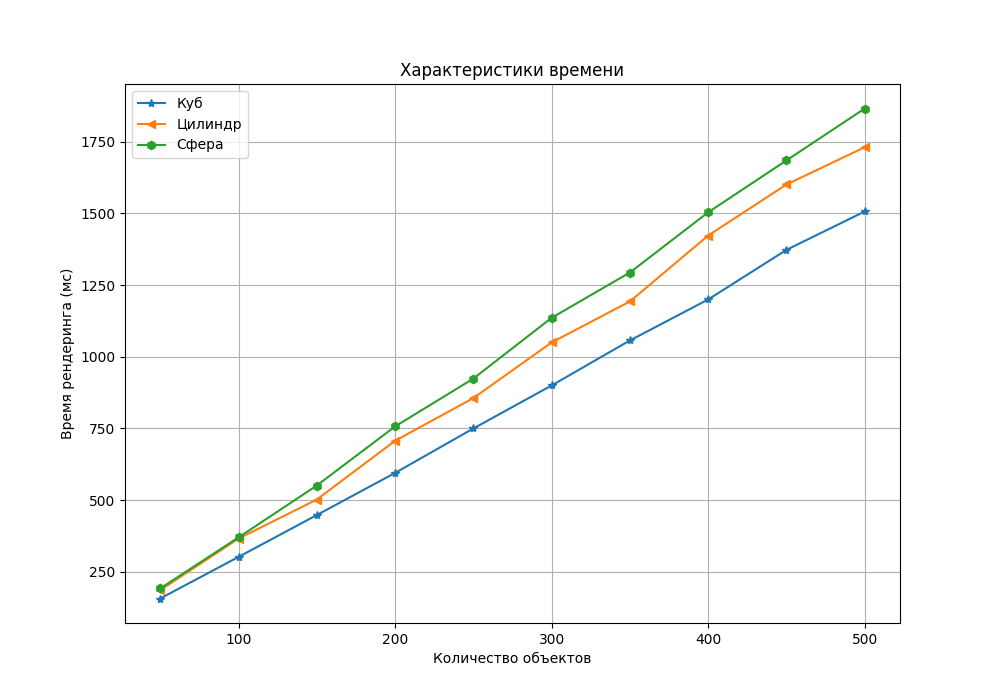
\includegraphics[width=0.9\textwidth]{img/exp/exp1.png}
	\caption{График зависимости времени отрисовки от числа объектов}
	\label{fig:exp-1}
\end{figure}

Как видно из графика, время визуализации сцены зависит от количества объектов линейно.

Следующим этапом исследования разработанной программы является исследование зависимости времени построения сцены от текстуры при фиксированном количестве объектов. В ходе исследования количество сфер менялось от 50 до 500 с шагом 50. 

\begin{figure}[h]
	\centering
	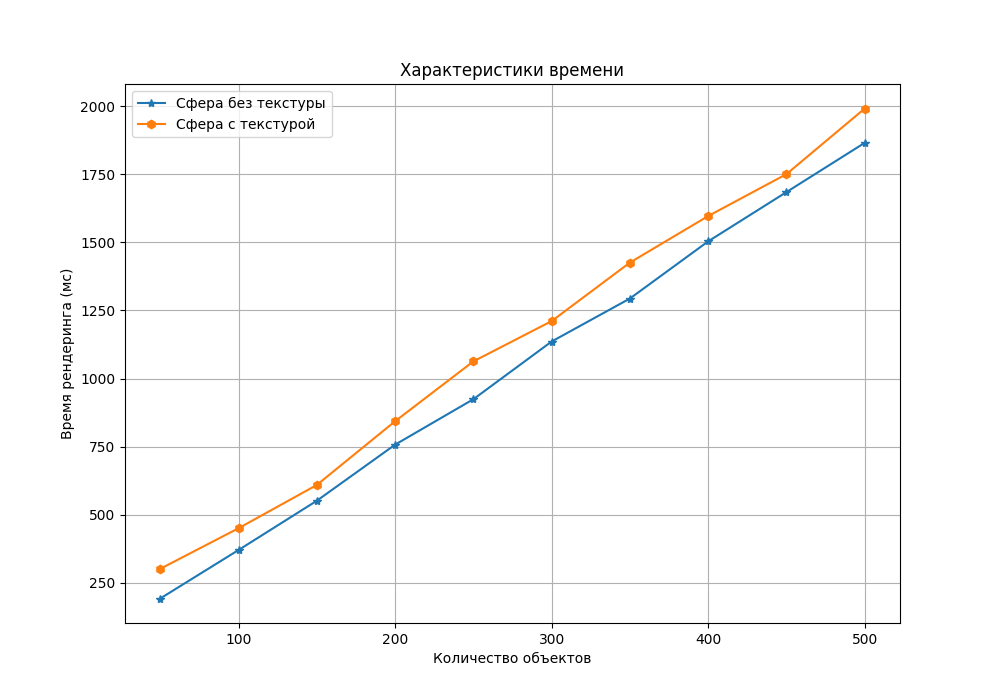
\includegraphics[width=0.9\textwidth]{img/exp/exp2.png}
	\caption{График зависимости времени отрисовки от учёта текстуры}
	\label{fig:exp-2}
\end{figure}
\clearpage
Из проведенного исследования можно сделать вывод, что время визуализации сцены линейно зависит от количества объектов на сцене. В случаях визуализации с учётом текстуры время растет объясняется сложностью при вычислении текстурных координат.

\subsection*{Вывод}
В данном разделе приведены результаты работы программного
обеспечения.

Результаты исследования совпали с ожидаемыми, так как в ходе исследования было установлено, что время работы увеличивается с увеличением количества объектов на сцене. Также время выполнения зависит от текстуры, которая накладывается на объект.